\ExplSyntaxOn
\int_gset:Nn \g__ptxcd_interlude_page_int {-1}
\ExplSyntaxOff

\interlude{What do we want?}

\begin{frame}[T]{}
  \centering
  \bsixonetwo

  { \footnotesize What do we want? }
  \\[-0.00cm] \resizebox{10cm}{!}{\bfseries \Large data communication}
  \\[.2cm] { \footnotesize How do we want it? }
  \\[-0.32cm] \resizebox{10cm}{!}{\bfseries \Large securely}
  \\[-0.15cm] { \footnotesize Specifically? }
  \\[.08cm] \resizebox{10cm}{!}{\bfseries \Large post-quantum secure}
\end{frame}
\begin{frame}[T]{}
  \begin{columns}[T,fullwidth]
    \begin{column}{.72\linewidth}
      \begin{tblr}{
        colspec = { r l c c c },
        cells   = { valign = m },
      }
        % HEADER: Encryption Technologies
          & % Image
          & \textbf{QKD}
          & \textbf{Guards}
          & \textbf{Crypto.}
        \\
        \adjustbox{valign=m}{\includegraphics[height=0.12\defaultframetextheight,trim=14 92 6 86,clip]{visualizations/comic/rosenpass-comic-qrn-mini-e2e.png}}
          &
          \begin{minipage}{0.2\textwidth}
            E2E Security
          \end{minipage}
          & \XSolidBrush
          & \Checkmark\textsuperscript{1}
          & \Checkmark
        \\
        \adjustbox{valign=m}{\includegraphics[height=0.2\defaultframetextheight,trim=4 77 4 55,clip]{visualizations/comic/rosenpass-comic-qrn-mini-auth.png}}
          &
          \begin{minipage}{0.2\textwidth}
            Auth.
          \end{minipage}
          & \Checkmark\textsuperscript{2}
          & \Checkmark\textsuperscript{1}
          & \Checkmark
        \\
        \adjustbox{valign=m}{\includegraphics[height=0.2\defaultframetextheight,trim=41 58 54 61,clip]{visualizations/comic/rosenpass-comic-qrn-mini-legacy.png}}
          &
          \begin{minipage}{0.2\textwidth}
            Commodity \\ Hardware
          \end{minipage}
          & \XSolidBrush
          & \XSolidBrush
          & \Checkmark
        \\
        \adjustbox{valign=m}{\includegraphics[height=0.2\defaultframetextheight,trim=15 50 22 42,clip]{visualizations/comic/rosenpass-comic-qrn-mini-datarates2.png}}
          &
          \begin{minipage}{0.2\textwidth}
            Data Rates
          \end{minipage}
          & kb
          & Any
          & Any
        \\
        \adjustbox{valign=m}{\includegraphics[height=0.2\defaultframetextheight,trim=40 50 40 50,clip]{visualizations/comic/rosenpass-comic-qrn-mini-hardness.png}}
          &
          \begin{minipage}{0.2\textwidth}
            Everlasting \\ Secrecy\textsuperscript{3}
          \end{minipage}
          & (\XSolidBrush)\textsuperscript{4}
          & (\Checkmark)\textsuperscript{1}
          & (\Checkmark)\textsuperscript{5}
      \end{tblr}
    \end{column}
    \begin{column}{.32\linewidth}
      \vspace{2em}
      \shiftbox{-.32\linewidth}{
        \begin{minipage}{\linewidth}
          \raggedright
          \footnotesize
          \textsuperscript{1}Assuming resistance against sneak attacks
          \\[0.4em] \textsuperscript{2}Through Wegman-Carter
          \\[0.4em] \textsuperscript{3}Information-Theoretic Security, the lack of algorithmic hardness assumptions
          \\[0.4em] \textsuperscript{4}Not at these data rates
          \\[0.4em] \textsuperscript{5}With a suitcase of hard drives containing keys
        \end{minipage}
      }
    \end{column}
  \end{columns}
\end{frame}

\begin{frame}[T]{}
  \centering
  \bsixonetwo
  { \small How to secure the internet against quantum attacks? }
  \\[0.3cm] \resizebox{14.3cm}{!}{\bfseries \Large With computational cryptography}
\end{frame}

\interlude{How do we think about QKD then?}

\begin{frame}[T]{Conceptualize QKD}
  \vspace{3em}
  \centering
  \shiftbox{-0.12\textwidth}{
    \includegraphics[width=1.20\textwidth,page=9,trim=95 340 90 590]{slide-graphics-qrn.pdf}
  }
  \\[1.5em] \textbf{QKD} as a measure of hardware security.
\end{frame}

\begin{frame}[T]{}
  \centering
  \includegraphics[height=1.15\defaultframetextheight,clip,trim=0 25 0 65]{scientific/rosenpass-qkd.pdf}
  \\ \textbf{QKD:} A fail-over in case Post-Quantum Cryptography fails.
\end{frame}

\begin{frame}[T]{}
  \centering
  \bsixonetwo

  { \footnotesize What do we want? }
  \\[-0.00cm] \resizebox{10cm}{!}{\bfseries \Large secure data communication}
  \\[.08cm] { \footnotesize Where do we want it? }
  \\[.2cm] \resizebox{10cm}{!}{\bfseries \Large on highly secure institutional networks}
  \\[.0cm] { \footnotesize In what particular manner? }
  \\[.00cm] \resizebox{10cm}{!}{\bfseries \Large with hardware security measures}
  \\[.08cm] \resizebox{10cm}{!}{\bfseries \Large especially QKD}
\end{frame}

\ExplSyntaxOn
\int_gset:Nn \g__ptxcd_interlude_page_int {-1}
\ExplSyntaxOff

\interlude{How do we build it?}

\begin{frame}[T]{How about a key management system?}
  \begin{columns}[T,fullwidth]
    \hfill
    \begin{column}{.45\linewidth}
      \centering
      \includegraphics[height=\defaultframetextheight,page=7,trim=1200 50 1200 130]{slide-graphics-qrn.pdf}
    \end{column}
    \begin{column}{.45\linewidth}
      \vspace{1.6em}
      \begin{itemize}
        \item Pretty expensive
        \item Pretty complicated
        \item Still requires IP-based networking
        \item One compromised node compromises the entire network
        \item Does not address how to create data channels
      \end{itemize}
    \end{column}
    \hfill
  \end{columns}
\end{frame}

\begin{frame}[T]{}
  \centering
  \includegraphics[height=1.2\defaultframetextheight]{comic/rosenpass-comic-rgm-3.png}
  \\[-0.6em] Key management systems evoke the image of a Rube Goldberg machine.
\end{frame}

\ExplSyntaxOn
\int_gset:Nn \g__ptxcd_interlude_page_int {-1}
\ExplSyntaxOff

\interlude{Back to the basics: What was the internet again?}

\begin{frame}[T]{}
  \centering
  \vspace{-2.3em}
  \includegraphics[height=0.6\defaultframetextheight]{visualizations/comic/rosenpass-comic-qrn-present}
  \\[-1em] The internet is \textbf{packet-routed} and \textbf{stateless}.

  \vspace{1.5em}
  \begin{minipage}[.4\pageheight]{\pagewidth}
    \only<1>{
      \shiftbox{-0.12\textwidth}{
        \includegraphics[width=0.985\textwidth,page=10,trim=95 340 90 440]{slide-graphics-qrn.pdf}
      }
      \\[0.2em] The internet is an architecture for \textbf{transport-agnostic} networking.
    }
    \only<2>{
      \shiftbox{-0.12\textwidth}{
        \includegraphics[width=0.985\textwidth,page=11,trim=95 340 90 440]{slide-graphics-qrn.pdf}
      }
      \\[0.2em] Then QKD is just another transport technology, with extra security features.
    }
  \end{minipage}
\end{frame}

\ExplSyntaxOn
\int_gset:Nn \g__ptxcd_interlude_page_int {-1}
\ExplSyntaxOff

\interlude{That's a wrap, problem solved!}

\begin{frame}[T]{}
  \centering
  \shiftbox{-0.1\textwidth}{
    \includegraphics[width=1.2\textwidth,page=4]{slide-graphics-qrn.pdf}
  }
  \\ To do this safely and securely, we need \textbf{secure routing} (for safety) and \textbf{E2E}-encryption (for security).
\end{frame}

\begin{frame}[T]{}
  \centering
  \shiftbox{-0.1\textwidth}{
    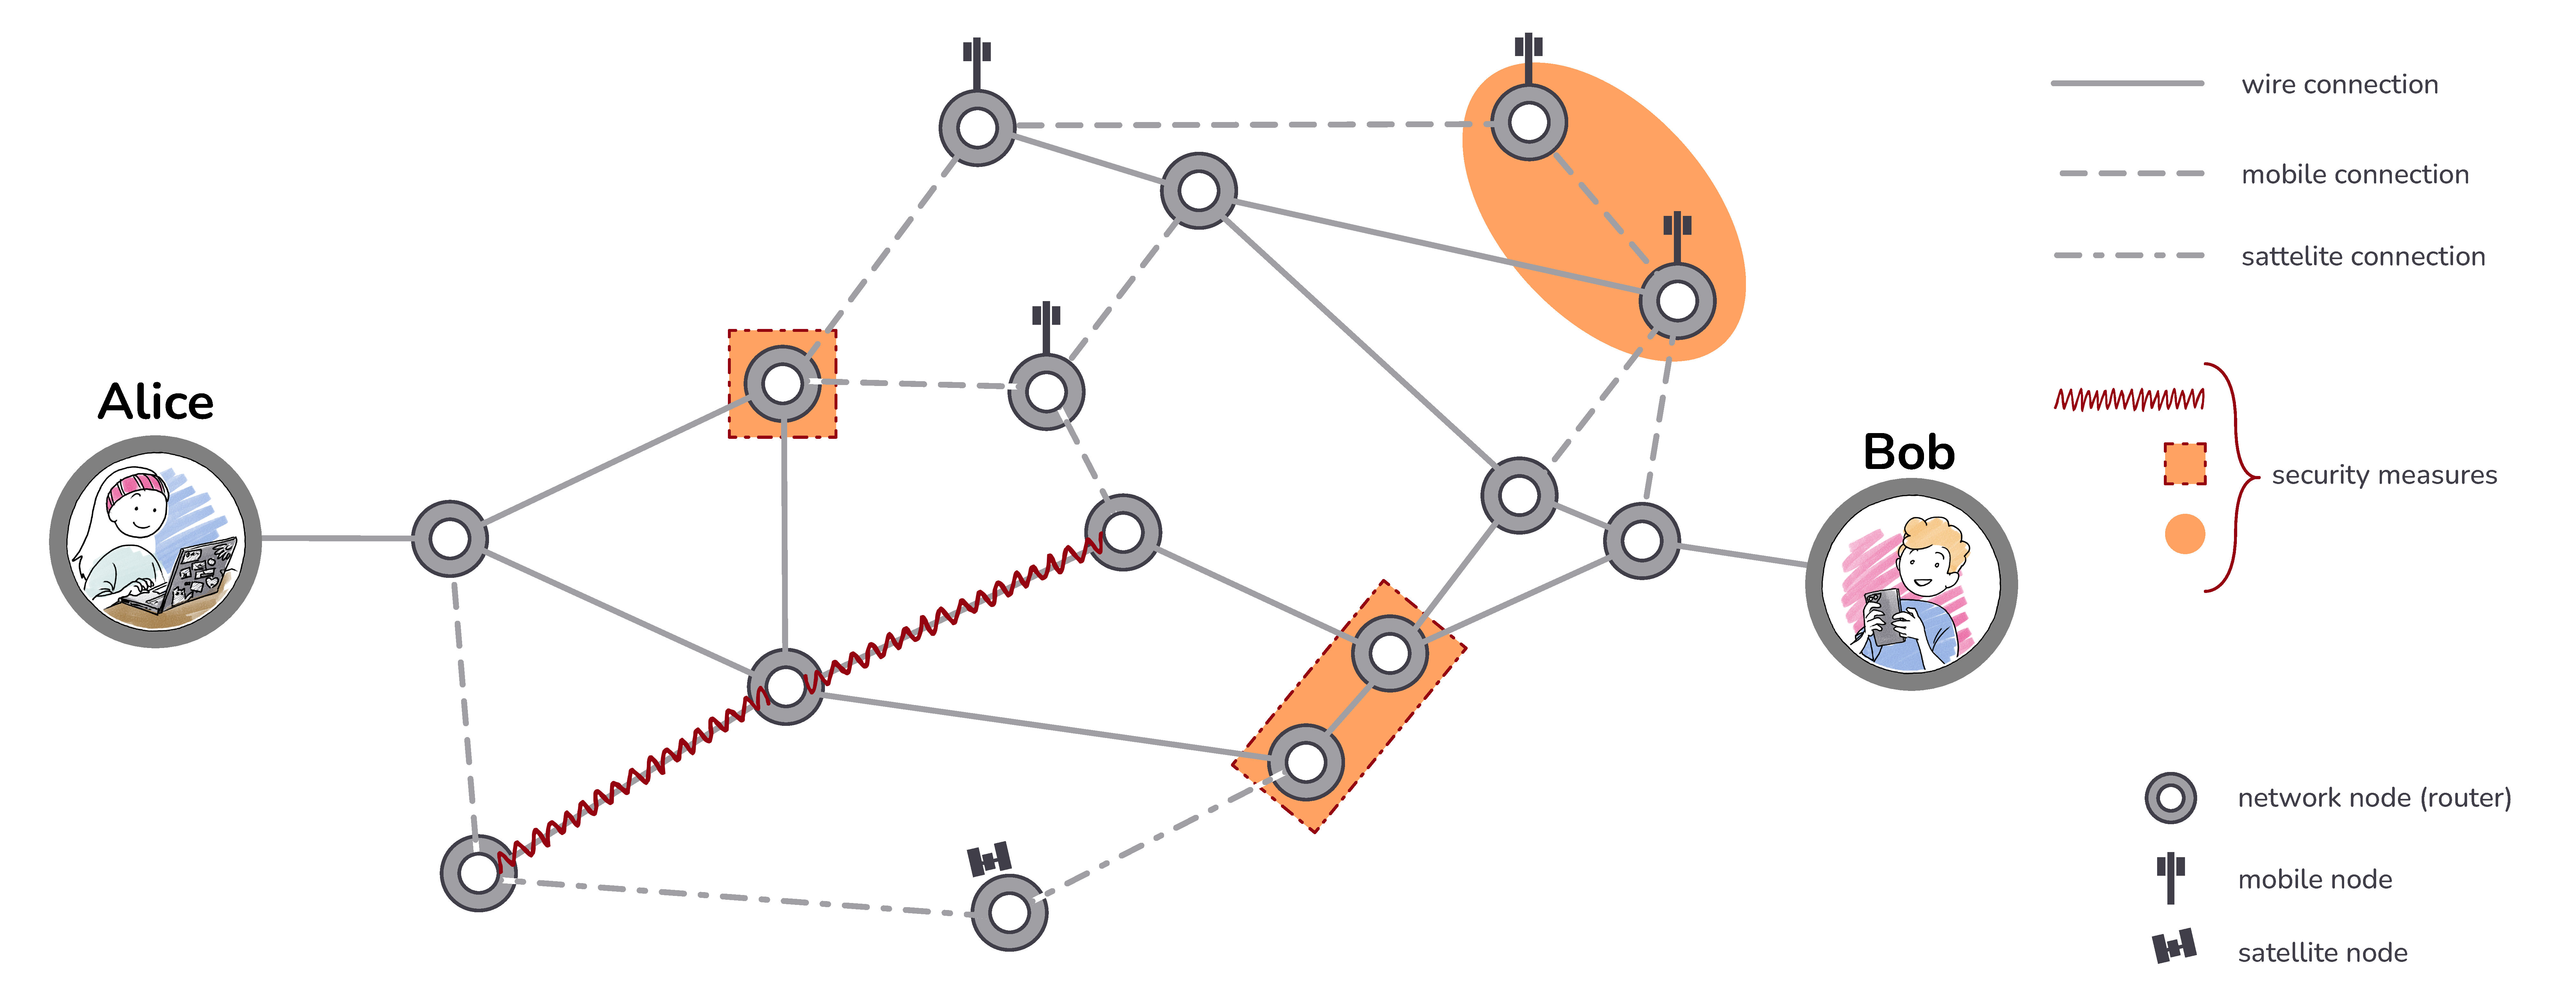
\includegraphics[width=1.2\textwidth,page=1]{slide-graphics-qrn.pdf}
  }
  \\ \textbf{Secure routing} detects and avoids \emph{accidentally insecure} routes.
\end{frame}

\begin{frame}[T]{}
  \begin{columns}[T,fullwidth]
    \begin{column}{.01\linewidth}
    \end{column}
    \begin{column}{.35\linewidth}
      \vspace{0.8em}
      With internet standard technologies:
      \begin{itemize}
        \item \textbf{SRv6} to fully control the routes packages take \\ … even if nodes not on the path are compromised.
        \item \textbf{HNCP} to learn the network topology \\ … and to automatically deploy networks in the first place.
      \end{itemize}
    \end{column}
    \begin{column}{.60\linewidth}
      \centering
      \shiftbox{-0.1\textwidth}{
        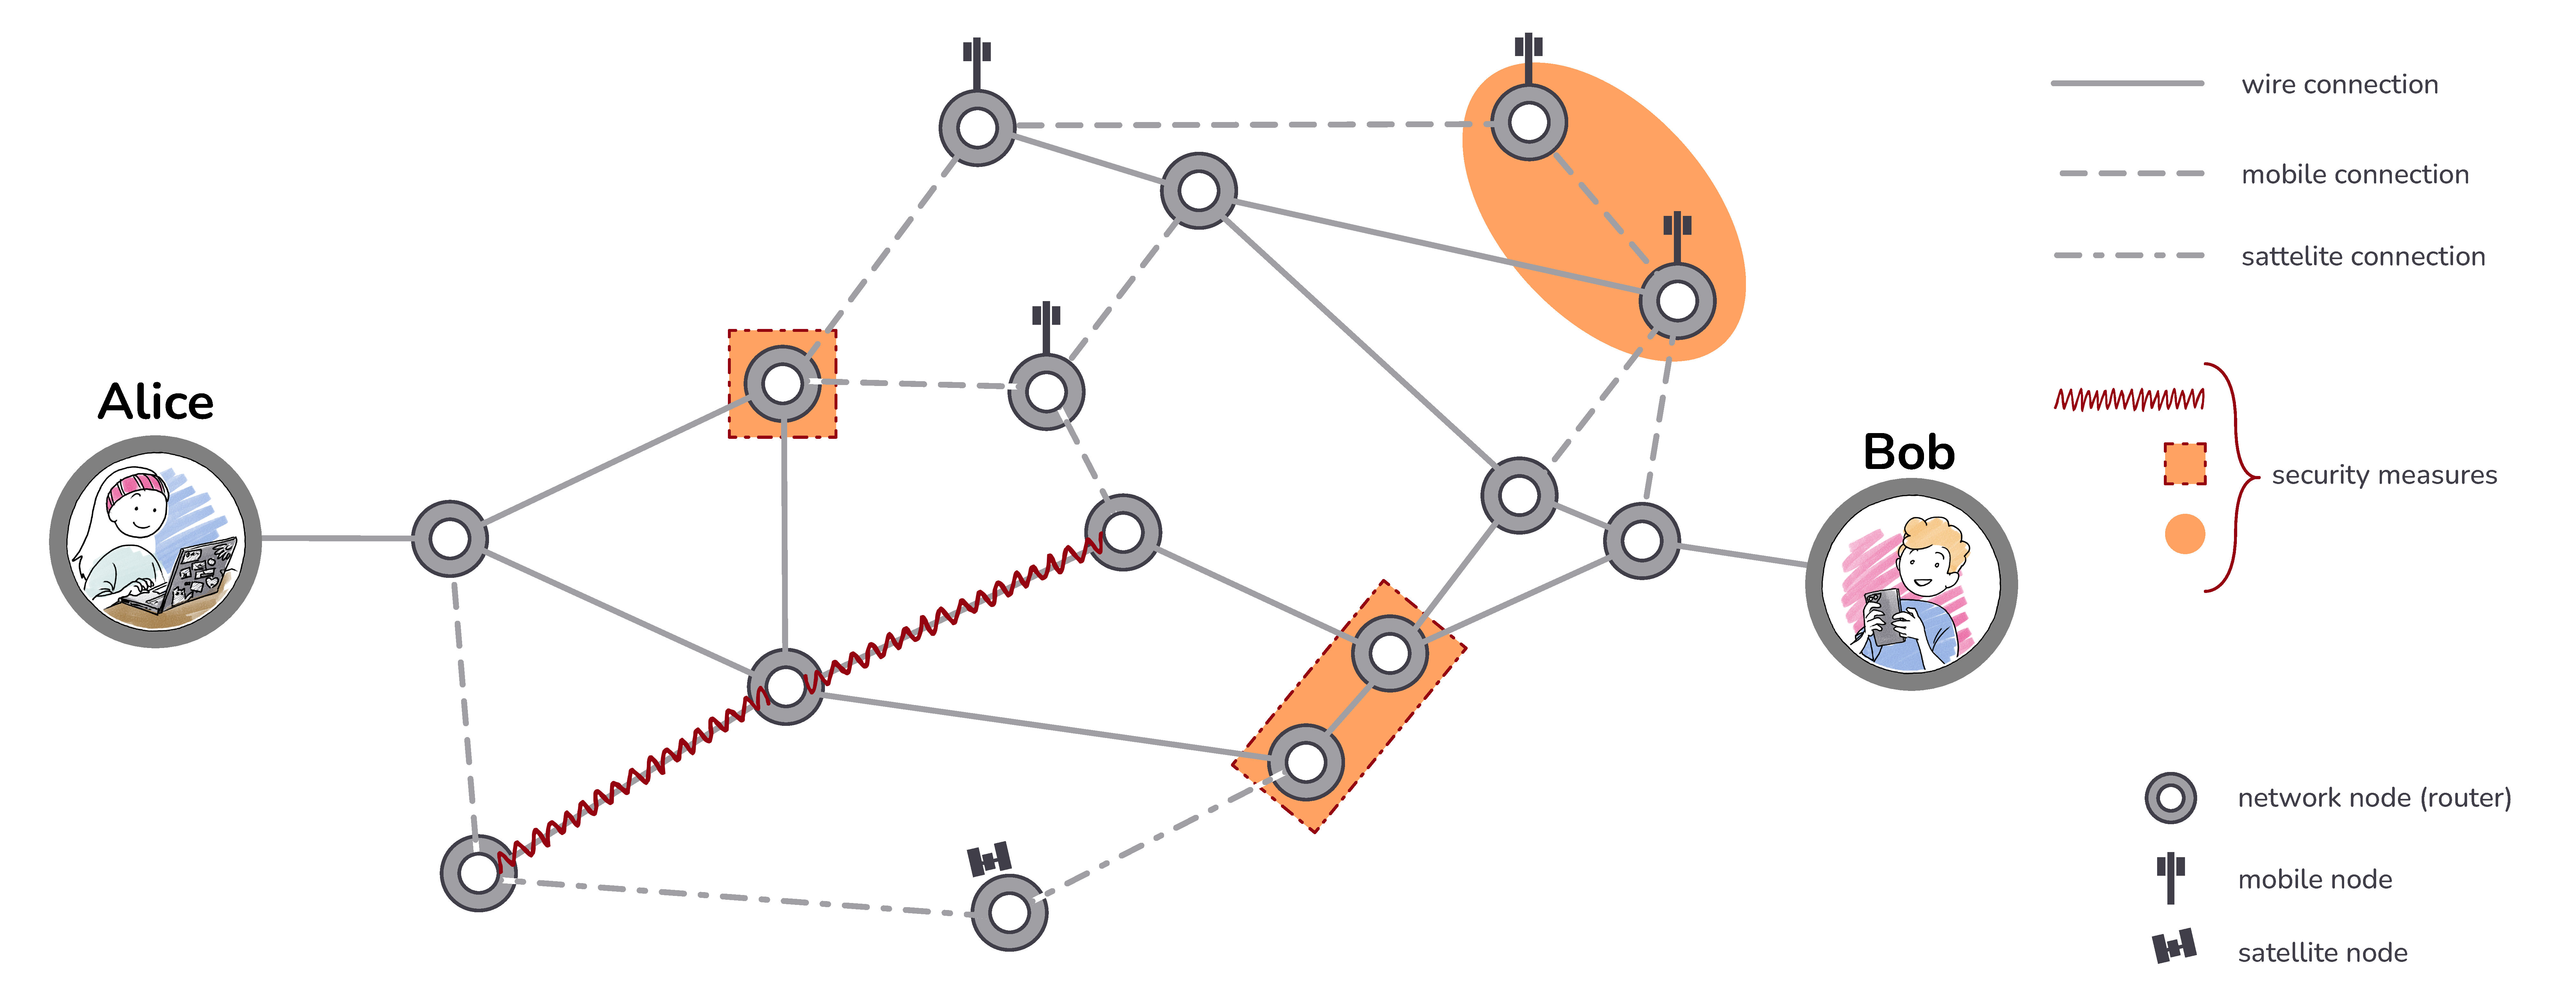
\includegraphics[height=0.8\defaultframetextheight,page=1,clip,trim=1300 0 0 0]{slide-graphics-qrn.pdf}
      }
      \\ \textbf{Secure routing} detects and avoids \emph{accidentally insecure} routes.
    \end{column}
  \end{columns}
\end{frame}

\begin{frame}[T]{}
  \centering
  \shiftbox{-0.1\textwidth}{
    \includegraphics[width=1.2\textwidth,page=2]{slide-graphics-qrn.pdf}
  }
  \\ And we need end-to-end cryptography for security.
  \\ For instance, using Rosenpass for post-quantum security and WireGuard for classical security.
\end{frame}

\begin{frame}[T]{}
  \centering
  \shiftbox{-0.1\textwidth}{
    \includegraphics[width=1.2\textwidth,page=3]{slide-graphics-qrn.pdf}
  }
  \\ Ingress-to-egress security can substitute for end-to-end security in corporate environments
  \\ … so the technology does not have to be installed on every old Windows laptop.
\end{frame}

\begin{frame}[T]{}
  \centering
  \shiftbox{-0.1\textwidth}{
    \includegraphics[width=1.2\textwidth,page=4]{slide-graphics-qrn.pdf}
  }
  \\ Here is what it might look like if a properly secure connection is established.
  \\ Note how secure routing invalidates the backup route, because it's not QKD secured all the way.
\end{frame}

\begin{frame}[T]{}
  \shiftbox{-0.08\textwidth}{
    KMS-Based Architecture\hspace{7.3em}Networking-oriented architecture
  }
  \shiftbox{-0.1\textwidth}{
    \includegraphics[width=1.15\textwidth,page=6,clip,trim=140 80 300 140]{slide-graphics-qrn.pdf}
  }
  \footnotesize
  \\[.6em]
  \shiftbox{-0.08\textwidth}{
    \begin{minipage}{.9\pagewidth}
      QKD becomes just another transport: SRv6, HNCP, and tunnels for added safety \& security.
      \\[.5em] \textbf{We now support}: automatic network deployment; hardware security other than QKD supported; 
      interoperability with the internet.
    \end{minipage}
  }
\end{frame}

\ExplSyntaxOn
\int_gset:Nn \g__ptxcd_interlude_page_int {-1}
\ExplSyntaxOff

\interlude{This is in fact a Key Management System}

\begin{frame}[T]{KMS by API adapter}
  \vspace{1em}
  \centering
  \shiftbox{-0.12\textwidth}{
    \includegraphics[width=1.20\textwidth,page=13,trim=95 340 90 200]{slide-graphics-qrn.pdf}
  }
  \small
  \\[.75em]
  \begin{minipage}{.9\pagewidth}
    \centering
    \textbf{Intuition:} Keys sent on a secured path gain the security properties of the secured path.
    \\[.8em] We can implement a KMS by exposing an API that chooses a random key, then transmits it.
    \\[.8em] The plan data path is almost always more useful.
  \end{minipage}
\end{frame}

\begin{frame}[T]{}
  \centering
  \shiftbox{-0.1\textwidth}{
    \includegraphics[width=1.2\textwidth,page=4]{slide-graphics-qrn.pdf}
  }
  \small
  \\[.75em]
  \begin{minipage}{.9\pagewidth}
    \centering
    \textbf{Information theoretic security:} No distinction; supported if the transports do support it.
    \\[.8em] (All transports must use One-Time-Pad with Wegman-Carter auth based on QKD-Keys).
  \end{minipage}
\end{frame}

\begin{frame}[T]{}
  \centering
  \shiftbox{-0.1\textwidth}{
    \includegraphics[width=1.2\textwidth,page=15]{slide-graphics-qrn.pdf}
  }
  \small
  \\[.75em]
  \begin{minipage}{.9\pagewidth}
    \centering
    \textbf{Quantum repeaters}: Just a special type of transport, no distinction for the network.
  \end{minipage}
\end{frame}

\interlude{What about a proper QKD-enabled internet?}

\begin{frame}[T]{}
  \centering
  \shiftbox{-0.1\textwidth}{
    \includegraphics[width=1.2\textwidth,page=5]{slide-graphics-qrn.pdf}
  }
  \small
  \\[.75em]
  \begin{minipage}{.9\pagewidth}
    \centering
    \textbf{Do not reinvent the wheel}; use established routing protocols:
    \\ Build an \textbf{extension to IPv6} that can transmit QKD keys alongside packages.
  \end{minipage}
\end{frame}

\interlude{Advertisement}

\begin{frame}{Collaborating with Quantum Optics Jena}
  \begin{columns}[fullwidth,c]
    \hspace*{.25\LeftSlideIndent}%
    \begin{column}{.45\linewidth}
      \centering
      \includegraphics[width=.82\linewidth]{visualizations/comic/rosenpass-comic-qrn-presents.png}
    \end{column}
    \begin{column}{\dimexpr.5\linewidth-.25\LeftSlideIndent}
      \vspace{0.6em}\textbf{WireGuard}: For classical security
      \\[.4em] \textbf{Rosenpass}: For post-quantum security
      \\[.4em] \textbf{QOJ QKD devices}: For QKD support
      \\[.4em] \textbf{HNCP}: For network observability and automatic network deployment.
      \\[.4em] \textbf{SRv6}: For secure routing support
      \\[1.2em] \shiftbox{-6em}{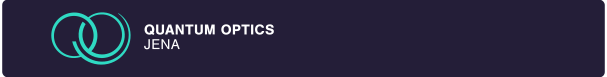
\includegraphics[height=4.5em,trim=0 0 240 0]{graphics/qoj.pdf}}
    \end{column}%
  \end{columns}
\end{frame}

\ExplSyntaxOn
\int_gset:Nn \g__ptxcd_interlude_page_int {-1}
\ExplSyntaxOff

\interlude{Key takeaways}

\begin{frame}[T]{}
  \begin{columns}[fullwidth,c]
    \hspace*{.25\LeftSlideIndent}%
    \begin{column}{\dimexpr.5\linewidth-.25\LeftSlideIndent}
      \small
      \vspace{8.2em}
      \begin{minipage}{\linewidth}
        \centering
        QKD is a hardware security measure. \\ Treat it as such.
        \\[.6em] Focus on connecting secure data paths; \\ build KMS on top if needed.
        \\[.6em] \textbf{Physicists, cryptographers, and network engineers must collaborate to build viable QKD-enabled networks.}
      \end{minipage}
      \\[2.8em]
      \begin{minipage}{\pagewidth}
        \footnotesize
        \shiftbox{-0.7em}{
          Rosenpass e. V.\ \textasciitilde\ rosenpass.eu
        }
        \\ \shiftbox{-0.7em}{
          Speaker: Karolin Varner (karo@rosenpass.eu)
        }
        \\ \shiftbox{-0.7em}{
          Scientific Illustration: Lisa Schmid (mullana@rosenpass.eu)
        }
      \end{minipage}
    \end{column}%
    \begin{column}{.45\linewidth}
      \includegraphics[height=.8\pageheight,trim=70 40 0 60]{visualizations/comic/rosenpass-comic-qrn-team.png}
    \end{column}
  \end{columns}
\end{frame}
